\section{VHDL}
Very High Speed Integrated Circuit Hardware Description Language.
It is a programming language that has been designed and optimized for describing
the behavior of digital systems.

\subsection{VHDL Syntax}

VHDL is not case sensitive, but it is a good practice to use upper case for keywords and lower case for everything else.
VHDL describes hardware and so instructions are executed in a concurrent manner, meaning that all instructions are executed at once.


Comments are written with two hyphens (- -).


\textbf{if, case and loop statements}

Every if statement has a corresponding then component and each if statement is terminated with an end if;
If an else if statement is needed then it can be written as elsif. Before
each if statement a process statement must be written. The process
statement includes the sensitivity list which is a list of signals that the process is sensitive to.

\begin{verbatim}
process (sel, I)
begin
  if (sel == "00") then
    a <= 'I';
    b <= '0';
    c <= '0';
    d <= '0';
      
  elsif (sel == "01") then
    a <= '0';
    b <= 'I';
    c <= '0';
    d <= '0';
  elsif (sel == "10") then
    a <= '0';
    b <= '0';
    c <= 'I';
    d <= '0';
  else
    a <= '0';
    b <= '0';
    c <= '0';
    d <= 'I';
  end if;
end process;
\end{verbatim}


Each case statement is terminated with end case; Each loop statement has a corresponding end loop;

\begin{verbatim}
case (expression) is
  when choices =>
    <sequential statements>
  when choices =>
    <sequential statements>
  when others =>
    <sequential statements>
end case;
\end{verbatim}


\textbf{Signal and variable assignments}

Among the most frequently used object types there is the signal object type, the variable object type, and the constant object type.
The signal type is the software representation of a wire in the digital system.
The variable type is used to store local information.
The constant type is used to store constant information.

Signals are declared at the top of the architecture body, just before the keyword begin.
Variables must be declared inside the process construct and are local.

Assigning a value to a signal is done using the signal assignment operator $<=$.
$$C <= not(A);$$
Assigning a value to a variable is done using the variable assignment operator $:=$.
$$ B := A;$$

A variable changes its value soon after the variable assignment is executed. Instead a signal
changes its value "some time" after the signal assignment expression is evaluated.


\subsection{VHDL Design Units}


\textbf{STD LOGIC}

\begin{center}
	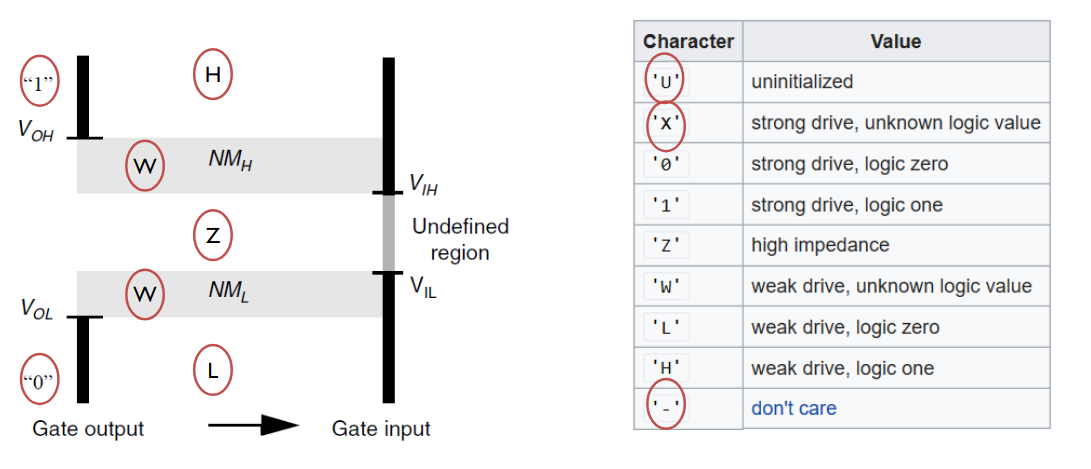
\includegraphics[width = 0.7\textwidth]{images/stdlogic.png}
\end{center}



\textbf{Entity}

The entity describes how the unit interfaces with the outside world.
The entity lists the various inputs and outputs of the underlying system.


\textbf{Architecture}

Describes what the circuit actually does. It describes the internal
implementation of the associated entity. An architecture can be written by means of three modeling
techniques plus any combination of these three: dataflow, behavioral, and structura plus any combination of these three.


\textbf{Karnaugh map (K-map)}

A method of circuit optimization. Aims to reduce logic functions
more quickly and easily compared to Boolean algebra.

\textbf{Combinational circuits}

It is defined as the time independent circuits which do not depend upon previous
inputs to generate any output.
e.g. Encoder, Decoder, Multiplexer, Demultiplexer etc.

\textbf{Sequential circuits}

Dependent on clock cycles and depends on present as well as past inputs to generate any output.
e.g. Flip-flops, Counters, Registers etc.


\textbf{Concurrent Statements}
CHDL has the ability to execute a virtually unlimited number of statements at the same time and in a concurrent manner. The key thing to remember is that we are
designing hardware.

\textbf{Conditional Signal Assignment when}

Conditional signal assignment is a concurrent statement that assigns a value to a signal based on the value of a condition. The syntax is:

\begin{verbatim}
  <target> <= <expression> when <condition> else 
          <expression> when <condition> else 
          <expression>;
\end{verbatim}

\textbf{Selected Signal Assignment with select}

Selected signal assignments only have one assignment operator. Selected signal assignment
differs from conditional assignment statements in that assignments are based upon the evaluation
of one expression. The syntax is:

\begin{verbatim}
  with <choose_expression> select
    <target> <= <expression> when <choices>,
                <expression> when <choices>
                <expression> when others;
\end{verbatim}

The general form of the selected signal assignment statement is similar to switch statements
as seen in algorithmic programming languages such as C.

\textbf{Process Statements}

The process statement is a stement which contains a certain number of instructions that, when the process statement
is executed, are executed sequentially. In other words the process statement is a tool that can be used
for executing a certain number of instructions in a sequential manner.

\textbf{Multiplexer}

A general multiplexer has n data inputs, one output, and m select inputs. The number of select inputs determines the number of data inputs. The number of select inputs determines the number of data inputs. The number of data inputs is 2 to the power of the number of select inputs.


\begin{center}
	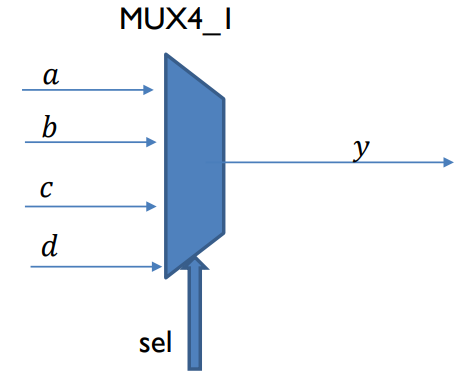
\includegraphics[width=0.3\textwidth]{images/mux.png}
\end{center}


\textbf{Demultiplexer}

It selects one ouput from the multiple output line and feteches the single input through
the selection line.


\begin{center}
	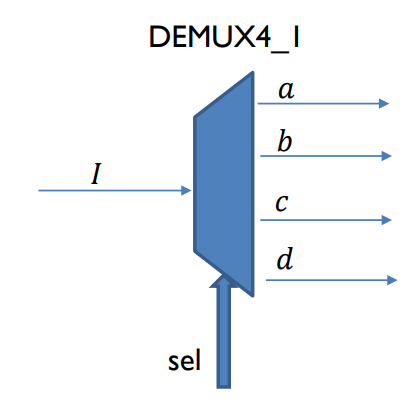
\includegraphics[width=0.2\textwidth]{images/demux.png}
\end{center}


\textbf{Encoders}

Encoders are used to encode data into a coded form and decoders
are used to convert it back into its original form. An encoder that has
$2^n$ input lines and n output lines is called an $n-to-2^n$ encoder.
It is assumed that only one input has a value of 1 at any given time.
It is used to minimize the number of input lines.

Priority encders are a modified version of an encoder. It gives a priority
to an input signal and provides an output based on that priority.

Example of a 4-to-2 priority encoder:

\begin{verbatim}
entity Priority_Encoder is
  port (D: in std_logic_vector(3 downto 0);
        Y: out std_logic_vector(1 downto 0));
end Priority_Encoder;

architecture Behavioral of Priority_Encoder is

begin
  process (D)
  begin
    if (D(3) = '1') then
      Y <= "11";
    elsif (D(2) = '1') then
      Y <= "10";
    elsif (D(1) = '1') then
      Y <= "01";
    elsif (D(0) = '1') then
      Y <= "00";
    else
      Y <= "---";
    end if;
  end process;
end Behavioral;
\end{verbatim}

\textbf{Decoders}

Decoders are used to decode data that has been encoded using a binary encoder.
An n-bit code can represent $2^n$ different values.
An encoder can be used with enable inputs. The enable inputs are used to enable or disable the decoder.

\newpage
\subsection{Standard models in VHDL Architecture}


\textbf{Data-flow style architecture}

Circuits are described by showing the input and ouput relationships between the various built-in components of the VHDL language.

\textbf{Behavioral style architecture}

It provides no details as to how the design is implemented in actual hardware.
The behavioral style models how the circuit outputs will react to the circuit inputs.
Whereas in data-flow modeling you somewhat need to have a feel for the underlying logic in the circuit.
In other words, data-flow modeling describes how the circuit should look in terms of logic gates
whereas behavioral modeling describes how the circuit should behave.
